\section{Estadísticas de números}

Escriba un programa que muestre la suma, el promedio, el máximo y el
mínimo de una secuencia de números.

El programa debe verse así:

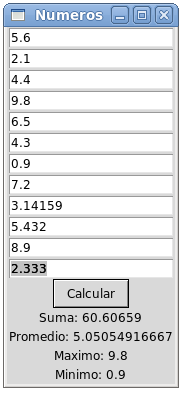
\includegraphics{../../diapos/programas/tkinter/capturas/09.png}

Al hacer clic en :kbd:`Calcular`, deben actualizarse los mensajes en la
parte inferior.

Es mala idea crear los modelos y los campos de entrada de la siguiente
manera:

\begin{lstlisting}
v1 = StringVar()
e1 = Entry(w, textvariable=v1)

v2 = StringVar()
e2 = Entry(w, textvariable=v2)

# ...
\end{lstlisting}

Un buen programador siempre busca la manera de evitar escribir código
repetitivo. Use ciclos y listas con este propósito.
